\documentclass[handout]{beamer}
\usetheme{metropolis}
\beamertemplatetransparentcoveredhigh

\usepackage[portuges]{babel}
\usepackage{graphicx}
\graphicspath{{./figs/}}
\usepackage{listings}
\usepackage{color}
\usepackage{hyperref}
\usepackage{xpatch}
\usepackage{comment}
\usepackage[outputdir=build]{minted}

\makeatletter
\AtBeginEnvironment{minted}{\dontdofcolorbox}
\def\dontdofcolorbox{\renewcommand\fcolorbox[4][]{##4}}
\xpatchcmd{\inputminted}{\minted@fvset}{\minted@fvset\dontdofcolorbox}{}{}
\xpatchcmd{\mintinline}{\minted@fvset}{\minted@fvset\dontdofcolorbox}{}{}
\makeatother
\setminted[c]{
  linenos=true,
  breaklines=true,
  encoding=utf8,
  frame=lines,
  framerule=0.5pt,
  autogobble,
  fontsize=\small,
}
\setminted[bash]{
  linenos=true,
  encoding=utf8,
  frame=lines,
  framerule=0.5pt,
  autogobble,
  fontsize=\small
}

\newcommand{\cod}[1]{\mintinline{c}{#1}}


\definecolor{dkgreen}{rgb}{0,0.6,0}
\definecolor{gray}{rgb}{0.5,0.5,0.5}
\definecolor{mauve}{rgb}{0.58,0,0.82}


\definecolor{Purple}{HTML}{911146}
\definecolor{Orange}{HTML}{CF4A30}
\setbeamercolor{alerted text}{fg=Orange}
\setbeamercolor{frametitle}{bg=Purple}
\setbeamercolor{block body}{bg=Purple!20,fg=black}
\setbeamercolor{block title}{bg=Purple!50,fg=black}
\setbeamertemplate{blocks}[rounded][shadow=true]


\newcounter{ExercicioCounter}
\newcommand{\exercicio}{\refstepcounter{ExercicioCounter} Exercício~\theExercicioCounter}

\newcommand{\setcoverbg}{
  \setbeamertemplate{background}
  {
\includegraphics[width=\paperwidth,height=\paperheight]{backgrounds/coverbg}}
}
\newcommand{\setsectionbg}{
  \setbeamertemplate{background}
  {
\includegraphics[width=\paperwidth,height=\paperheight]{backgrounds/blank}}
}

\title{Programação Estruturada}
\subtitle{Arquivos}

\author{Professores Emílio Francesquini e Carla Negri Lintzmayer}
\institute{Centro de Matemática, Computação e Cognição\\ Universidade
  Federal do ABC} \date{2018.Q3}

\begin{document}

\setcoverbg
\maketitle
\setsectionbg


%%%%%%%%%%%%%%%%%%%%%%%%%%%%%%%%%%%%%%%%%%%%
%%%%%%%%%%%%%%%%%%%%%%%%%%%%%%%%%%%%%%%%%%%%
%%%%%%%%%%%%%%%%%%%%%%%%%%%%%%%%%%%%%%%%%%%%
%%%%%%%%%%%%%%%%%%%%%%%%%%%%%%%%%%%%%%%%%%%%
%%%%%%%%%%%%%%%%%%%%%%%%%%%%%%%%%%%%%%%%%%%%
%%%%%%%%%%%%%%%%%%%%%%%%%%%%%%%%%%%%%%%%%%%%
\section{Parâmetros do programa: argc e argv}

%%%%%%%%%%%%%%%%%%%%%%%%%%%%%%%%%%%%%%%%%%%%
\begin{frame}[fragile]{Argc e argv}

    \begin{itemize}
        \item Até então temos criado programas onde a função \cod{main()} não tem parâmetros.
        \item Mas esta função pode receber dois parâmetros: \cod{main(int argc, char *argv[])}.
        \begin{itemize}
            \item \cod{argc} (\emph{argument counter}): indica o número de argumentos na linha de comando ao se executar o programa.
            \item \cod{*argv[]} (\emph{argument vector}): é um vetor de ponteiros para caracteres (ou seja vetor de strings) que contém os argumentos da linha de comando, um em cada posição do vetor.
        \end{itemize}
    \end{itemize}

\end{frame}

%%%%%%%%%%%%%%%%%%%%%%%%%%%%%%%%%%%%%%%%%%%%
\begin{frame}[fragile]{Argc e argv}

    O programa abaixo imprime cada um dos parâmetros passados na linha de comando:
    \begin{minted}{c}
        #include <stdio.h>

        int main(int argc, char *argv[]) {
            int i;
            for (i = 0; i < argc; i++) {
                printf("%s\n", argv[i]);
            }
            return 0;
        }
    \end{minted}

\end{frame}

%%%%%%%%%%%%%%%%%%%%%%%%%%%%%%%%%%%%%%%%%%%%
\begin{frame}[fragile]{Argc e argv}

    \begin{itemize}
        \item Seu uso é útil em programas onde dados de entrada são passados via linha de comando.
        \item Exemplo: dados a serem processados estão em um arquivo, cujo nome é passado na linha de comando.
    \end{itemize}

    \begin{minted}[fontsize=\scriptsize]{c}
        #include <stdio.h>

        int main(int argc, char *argv[]) {
            if (argc < 2)
                printf("Informe o nome do arquivo.\n");
            else
                printf("Arquivo a ser processado: %s\n", argv[1]);
            return 0;
        }
    \end{minted}

\end{frame}

%%%%%%%%%%%%%%%%%%%%%%%%%%%%%%%%%%%%%%%%%%%%
%%%%%%%%%%%%%%%%%%%%%%%%%%%%%%%%%%%%%%%%%%%%
%%%%%%%%%%%%%%%%%%%%%%%%%%%%%%%%%%%%%%%%%%%%
%%%%%%%%%%%%%%%%%%%%%%%%%%%%%%%%%%%%%%%%%%%%
%%%%%%%%%%%%%%%%%%%%%%%%%%%%%%%%%%%%%%%%%%%%
%%%%%%%%%%%%%%%%%%%%%%%%%%%%%%%%%%%%%%%%%%%%
\section{Arquivos}

%%%%%%%%%%%%%%%%%%%%%%%%%%%%%%%%%%%%%%%%%%%%
%%%%%%%%%%%%%%%%%%%%%%%%%%%%%%%%%%%%%%%%%%%%
%%%%%%%%%%%%%%%%%%%%%%%%%%%%%%%%%%%%%%%%%%%%
\subsection{Introdução a arquivos em C}

%%%%%%%%%%%%%%%%%%%%%%%%%%%%%%%%%%%%%%%%%%%%
\begin{frame}{Tipos de memória}

    \begin{itemize}
        \item Quando vimos a organização básica de um sistema computacional, havia
        somente um tipo de memória.
        \item Mas na maioria dos sistemas, a memória é dividida em dois tipos:
    \end{itemize}
    \vspace{-1em}
    \begin{center}
        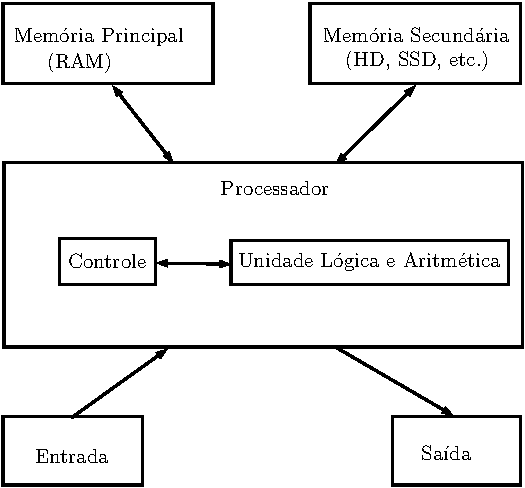
\includegraphics[scale=0.7]{organizacao}
    \end{center}

\end{frame}

%%%%%%%%%%%%%%%%%%%%%%%%%%%%%%%%%%%%%%%%%%%%
\begin{frame}{Tipos de memória}

    A memória principal (Random Access Memory) utilizada na maioria dos
    computadores, usa uma tecnologia que requer alimentação constante de
    energia para que informações sejam preservadas.

    \begin{center}
        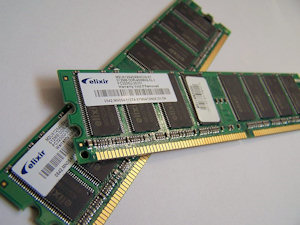
\includegraphics[scale=0.7]{ram}
    \end{center}

\end{frame}

%%%%%%%%%%%%%%%%%%%%%%%%%%%%%%%%%%%%%%%%%%%%
\begin{frame}{Tipos de memória}

    A memória secundária (como Hard Disks ou SSD) utilizada na maioria dos
    computadores, usa uma outra tecnologia que NÃO requer alimentação constante
    de energia para que informações sejam preservadas.

    \begin{center}
        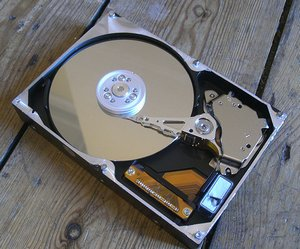
\includegraphics[scale=0.6]{hard_drive}
    \end{center}

\end{frame}

%%%%%%%%%%%%%%%%%%%%%%%%%%%%%%%%%%%%%%%%%%%%
\begin{frame}{Tipos de memória}

    \begin{itemize}
        \item Todos os  programas executam na RAM, e por isso quando o programa termina
        ou acaba energia, as informações do programa são perdidas.
        \pause
        \item Para podermos gravar informações de forma {\it persistente}, devemos escrever
        estas informações em arquivos na memória secundária.
        \pause
        \item A memória secundária possui algumas características:
        \begin{itemize}
            \item É muito mais lenta que a RAM.
            \item É muito mais barata que a memória RAM.
            \item Possui maior capacidade de armazenamento.
        \end{itemize}
        \pause
        \item Sempre que nos referirmos a um arquivo, estamos falando de informações
        armazenadas em memória secundária.
    \end{itemize}

\end{frame}

%%%%%%%%%%%%%%%%%%%%%%%%%%%%%%%%%%%%%%%%%%%%
%%%%%%%%%%%%%%%%%%%%%%%%%%%%%%%%%%%%%%%%%%%%
%%%%%%%%%%%%%%%%%%%%%%%%%%%%%%%%%%%%%%%%%%%%
\subsection{Nomes e extensões}

%%%%%%%%%%%%%%%%%%%%%%%%%%%%%%%%%%%%%%%%%%%%
\begin{frame}{Nomes e extensões}

    \begin{itemize}
        \item Arquivos são identificados por um nome.
        \item O nome de um arquivo pode conter uma extensão que indica o
        conteúdo do arquivo.
    \end{itemize}

    \begin{block}{Algumas extensões}
        \begin{center}
            \begin{tabular}{| l | l | } \hline
              arq.txt & arquivo texto simples \\\hline
              arq.c & código fonte em C\\\hline
              arq.pdf & \textsl{portable document format}\\\hline
              arq.html & arquivo para páginas WWW \\
                      & \textsl{(hypertext markup language)}\\\hline
              arq$^*$ & arquivo executável (UNIX) \\\hline
              arq.exe & arquivo executável (Windows) \\\hline
            \end{tabular}
        \end{center}
    \end{block}

\end{frame}

%%%%%%%%%%%%%%%%%%%%%%%%%%%%%%%%%%%%%%%%%%%%
%%%%%%%%%%%%%%%%%%%%%%%%%%%%%%%%%%%%%%%%%%%%
%%%%%%%%%%%%%%%%%%%%%%%%%%%%%%%%%%%%%%%%%%%%
\subsection{Tipos de arquivos}

%%%%%%%%%%%%%%%%%%%%%%%%%%%%%%%%%%%%%%%%%%%%
\begin{frame}{Tipos de arquivos}

    Arquivos podem ter o mais variado conteúdo, mas do ponto de vista
    dos programas existem apenas dois tipos de arquivo:

    \begin{block}{}
        \begin{description}
            \item[Arquivo texto:] Armazena caracteres que podem ser mostrados
            diretamente na tela ou modificados por um editor de textos
            simples. Exemplos: código fonte C, documento texto simples,
            páginas HTML.

            \item[Arquivo binário:] Sequência de bits sujeita às convenções
            dos programas que o gerou, não legíveis diretamente.  Exemplos:
            arquivos executáveis, arquivos compactados, documentos do Word.
        \end{description}
    \end{block}

\end{frame}

%%%%%%%%%%%%%%%%%%%%%%%%%%%%%%%%%%%%%%%%%%%%
%%%%%%%%%%%%%%%%%%%%%%%%%%%%%%%%%%%%%%%%%%%%
%%%%%%%%%%%%%%%%%%%%%%%%%%%%%%%%%%%%%%%%%%%%
\subsection{Caminhos absolutos e relativos}

%%%%%%%%%%%%%%%%%%%%%%%%%%%%%%%%%%%%%%%%%%%%
\begin{frame}[fragile]{Diretório}

    \begin{itemize}
        \item Também chamado de pasta.
        \item Contém arquivos e/ou outros diretórios.
    \end{itemize}
    \begin{block}{Uma hierarquia de diretórios}

\begin{verbatim}
               /                 diretório raiz
          /         \
       home         bin          subdiretórios
      /   \        /   \
   usr1   usr2    kate  emacs
  /    \
arq.txt mc102
         \
         lab.c
\end{verbatim}
    \end{block}

\end{frame}

%%%%%%%%%%%%%%%%%%%%%%%%%%%%%%%%%%%%%%%%%%%%
\begin{frame}[fragile]{Caminhos absolutos e relativos}

    \begin{itemize}
        \item  O nome de um arquivo pode conter o seu diretório, ou seja, o caminho
        para encontrar este arquivo a partir da raiz.
        \item Desta forma  o acesso a um arquivo pode ser
        especificado de duas formas:

        \begin{block}{}
            \begin{description}
                \item[Caminho absoluto:] descrição de um caminho desde o diretório raiz.
\begin{verbatim}
/bin/emacs
/home/usr1/arq.txt
\end{verbatim}
                \item[Caminho relativo:] descrição de um caminho a partir  do diretório
                corrente.
\begin{verbatim}
arq.txt
mc102/lab.c
\end{verbatim}
            \end{description}
        \end{block}

    \end{itemize}

    % Para ver qual é o diretório corrente, use o comando \texttt{pwd}. Para
    % mudar de diretório, use o comando \texttt{cd}.
\end{frame}

%%%%%%%%%%%%%%%%%%%%%%%%%%%%%%%%%%%%%%%%%%%%
% \begin{frame}
%     \frametitle{Atributos de arquivos}

%     Além do nome, arquivos possuem vários outros atributos:

%     \begin{block}{}
%         \begin{itemize}
%             \item Nome do arquivo
%             \item Proprietário do arquivo
%             \item Datas de criação, alteração e acesso
%             \item Tamanho em bytes
%             \item Permissão de acesso
%         \end{itemize}
%     \end{block}

%     Para ver estes atributos, use os comandos \texttt{ls -l} e \texttt{stat}.
% \end{frame}


% \begin{frame}[fragile]
%     \frametitle{Permissão de acesso}

%     Existem três níveis de controle: proprietário, grupo e todos.

%     \begin{minted}{c}
%         $ ls -l
%         -rw-r----- 1 jose alunos  545 Nov  8  2005 cp.c
%         drwxr-xr-x 2 jose alunos 4096 Jun  6 14:54 mc102/
%     \end{minted}

%     \begin{block}{}
%         \begin{itemize}
%             \item r: leitura
%             \item w: escrita
%             \item x: execução para arquivos, permissão de entrada para
%             diretórios
%         \end{itemize}
%     \end{block}
% \end{frame}

%%%%%%%%%%%%%%%%%%%%%%%%%%%%%%%%%%%%%%%%%%%%
%%%%%%%%%%%%%%%%%%%%%%%%%%%%%%%%%%%%%%%%%%%%
%%%%%%%%%%%%%%%%%%%%%%%%%%%%%%%%%%%%%%%%%%%%
%%%%%%%%%%%%%%%%%%%%%%%%%%%%%%%%%%%%%%%%%%%%
%%%%%%%%%%%%%%%%%%%%%%%%%%%%%%%%%%%%%%%%%%%%
%%%%%%%%%%%%%%%%%%%%%%%%%%%%%%%%%%%%%%%%%%%%
\section{Arquivos textos}

%%%%%%%%%%%%%%%%%%%%%%%%%%%%%%%%%%%%%%%%%%%%
%%%%%%%%%%%%%%%%%%%%%%%%%%%%%%%%%%%%%%%%%%%%
%%%%%%%%%%%%%%%%%%%%%%%%%%%%%%%%%%%%%%%%%%%%
\subsection{Ponteiro para arquivos}

%%%%%%%%%%%%%%%%%%%%%%%%%%%%%%%%%%%
\begin{frame}[fragile]{Arquivos texto em C}

    \begin{itemize}
        \item Em C, para se trabalhar com arquivos devemos criar um ponteiro especial: \textbf{um ponteiro para arquivos.}
        % begin{block}{}
        \begin{minted}[linenos=false]{c}
            FILE *nome_variavel;
        \end{minted}
        % \end{block}
        \item O comando acima cria um ponteiro para arquivos, cujo nome da variável é o nome especificado.
    \end{itemize}
    \begin{itemize}
        \item Após ser criado um ponteiro para arquivo, podemos associá-lo com um arquivo real do computador
        usando a função \textbf{fopen}.
        \begin{minted}[linenos=false]{c}
            FILE *arq1;
            arq1 = fopen("teste.txt", "r");
        \end{minted}
    \end{itemize}

\end{frame}

%%%%%%%%%%%%%%%%%%%%%%%%%%%%%%%%%%%
\begin{frame}[fragile]{Arquivos texto em C}

    \begin{minted}{c}
        FILE *arq1;
        arq1 = fopen("teste.txt", "r");
    \end{minted}
    \begin{itemize}
        \item O primeiro parâmetro para \textbf{fopen} é uma string com o nome do arquivo
        \begin{itemize}
            \item Pode ser absoluto, por exemplo: "/user/eduardo/teste.txt"
            \item Pode ser relativo como no exemplo acima: "teste.txt"
        \end{itemize}
        \item O segundo parâmetro é uma string informando como o arquivo será aberto.
        \begin{itemize}
            \item Se para leitura ou gravação de dados, ou ambos.
            \item Se é texto ou se é binário.
            \item No nosso exemplo, o \textbf{``r''} significa que abrimos um arquivo texto para leitura.
        \end{itemize}
    \end{itemize}
\end{frame}

%%%%%%%%%%%%%%%%%%%%%%%%%%%%%%%%%%%%%%%%%%%%
%%%%%%%%%%%%%%%%%%%%%%%%%%%%%%%%%%%%%%%%%%%%
%%%%%%%%%%%%%%%%%%%%%%%%%%%%%%%%%%%%%%%%%%%%
\subsection{Abrindo um arquivo}

%%%%%%%%%%%%%%%%%%%%%%%%%%%%%%%%%%%%%%%
\begin{frame}[fragile]{Abrindo um arquivo texto para leitura}
    \begin{itemize}
        \item Antes de acessar um arquivo, devemos abri-lo com a função
        \texttt{fopen()}.
        \item A função retorna um ponteiro para o arquivo em
        caso de sucesso, e em caso de erro a função retorna \texttt{NULL}.

        \item Abrindo o arquivo \texttt{teste.txt}:
        \begin{minted}{c}
            FILE *arq = fopen("teste.txt", "r");
            if (arq == NULL)
                printf("Erro ao tentar abrir o arquivo teste.txt.\n");
            else
                printf("Arquivo aberto para leitura.\n");
        \end{minted}
    \end{itemize}

\end{frame}

%%%%%%%%%%%%%%%%%%%%%%%%%%%%%%%%%%%%%%%%%%%%
%%%%%%%%%%%%%%%%%%%%%%%%%%%%%%%%%%%%%%%%%%%%
%%%%%%%%%%%%%%%%%%%%%%%%%%%%%%%%%%%%%%%%%%%%
\subsection{Lendo um arquivo}

%%%%%%%%%%%%%%%%%%%%%%%%%%%%%%%
\begin{frame}[fragile]{Lendo dados de um arquivo texto}

    \begin{itemize}

        \item Para ler dados do arquivo aberto, usamos a função \textbf{fscanf()}, que é
        semelhante à função \textbf{scanf()}.
        \begin{itemize}
            \item \textbf{int fscanf(ponteiro para arquivo, string de formato, variáveis)}.
            \item A única diferença para o \textbf{scanf}, é que devemos passar como primeiro parâmetro
            um ponteiro para o arquivo de onde será feita a leitura.
        \end{itemize}

        \item Lendo dados do arquivo \texttt{teste.txt}:
        \begin{minted}{c}
            char aux;
            FILE *f = fopen("teste.txt", "r");
            fscanf(f, "%c", &aux);
            printf("%c", aux);
        \end{minted}
    \end{itemize}

\end{frame}

%%%%%%%%%%%%%%%%%%%%%%%%%%%%%%%
\begin{frame}[fragile]{Lendo dados de um arquivo texto}

    \begin{itemize}
        \item Quando um arquivo é aberto, um \textbf{indicador de posição} no arquivo é criado, e este
        recebe a posição do início do arquivo.
        \item Para cada dado lido do arquivo, este indicador de posição é automaticamente incrementado
        para o próximo dado não lido.
        \item Eventualmente o indicador de posição pode chegar ao fim do arquivo:
        \begin{itemize}
            \item A função \textbf{fscanf} devolve um valor especial, \textbf{EOF} ({\it End Of File}), caso tente-se
            ler dados e o indicador de posição está no fim do arquivo.
        \end{itemize}
    \end{itemize}

\end{frame}

%%%%%%%%%%%%%%%%%%%%%%%%%%%%%%%
\begin{frame}[fragile]{Lendo dados de um arquivo texto}

    \begin{itemize}
        \item Para ler todos os dados de um arquivo texto, basta usarmos um laço
        que será executado enquanto não chegarmos no fim do arquivo.

        \item Lendo dados do arquivo \texttt{teste.txt}:
        \begin{minted}{c}
            char aux;
            FILE *f = fopen("teste.txt", "r");
            while (fscanf(f, "%c", &aux) != EOF)
                printf("%c", aux);
            fclose(f);
        \end{minted}

        \item O comando \textbf{fclose} (no fim do código) deve sempre ser usado para fechar um arquivo que foi aberto.
        \begin{itemize}
            \item Quando escrevemos dados em um arquivo, este comando garante que os dados serão
            efetivamente escritos no arquivo.
        \end{itemize}
    \end{itemize}

\end{frame}

%%%%%%%%%%%%%%%%%%%%%%%%%%%%%%%%%%%%%%%
\begin{frame}[fragile]{Lendo dados de um arquivo texto: exemplo}

    Programa que imprime o conteúdo de um arquivo passado como parâmetro do programa:

    \begin{minted}[fontsize=\scriptsize]{c}
        #include <stdio.h>
        int main(int argc, char *argv[]) {
            FILE *arq;
            char aux;
            if (argc <2) {
                printf("Informe o nome do arquivo.\n");
                return 1;
            }
            arq = fopen(argv[1], "r");
            if (arq == NULL) {
                printf("Problema ao ler o arquivo.\n");
                return 1;
            }
            while (fscanf(arq, "%c", &aux) != EOF) {
                printf("%c", aux);
            }
            fclose(arq);
            return 0;
        }
    \end{minted}

\end{frame}

%%%%%%%%%%%%%%%%%%%%%%%%%%%%%%%
\begin{frame}[fragile]{Lendo dados de um arquivo texto}

    \begin{itemize}
        \item Notem que ao realizar a leitura de um caractere, automaticamente
        o indicador de posição do arquivo se move para o próximo caractere.
        \item Ao chegar no fim do arquivo a função \textbf{fscanf} retorna o valor
        especial \textbf{EOF}.
        \item Para voltar ao início do arquivo você pode
        fechá-lo e abrí-lo mais uma vez, ou usar o comando \textbf{rewind}.
        \begin{minted}{c}
            while (fscanf(arq, "%c", &aux) != EOF)
                printf("%c", aux);

            printf("\n\n -----Imprimindo novamente\n\n");
            rewind(arq);

            while (fscanf(arq, "%c", &aux) != EOF)
                printf("%c", aux);
      \end{minted}
  \end{itemize}

\end{frame}


%%%%%%%%%%%%%%%%%%%%%%%%%%%%%%%%%%%%%%%%%%%%
%%%%%%%%%%%%%%%%%%%%%%%%%%%%%%%%%%%%%%%%%%%%
%%%%%%%%%%%%%%%%%%%%%%%%%%%%%%%%%%%%%%%%%%%%
\subsection{Escrevendo em um arquivo}

%%%%%%%%%%%%%%%%%%%%%%%%%%%%%%
\begin{frame}[fragile]{Escrevendo dados em um arquivo texto}

    \begin{itemize}
        \item Para escrever em um arquivo, ele deve ser aberto de forma
        apropriada, usando a opção \textbf{w}.
        \item Usamos a função \textbf{fprintf()}, semelhante à função
        \textbf{printf()}.
        \begin{itemize}
            \item \textbf{int fprintf(ponteiro para arquivo, string de saída, variáveis)}
            \item É semelhante ao \textbf{printf} mas notem que precisamos passar
            o ponteiro para o arquivo onde os dados serão escritos.
        \end{itemize}

        \item Copiando dois arquivos:
         \begin{minted}{c}
            FILE *arqin = fopen("entrada.txt", "r");
            FILE *arqout = fopen("saida.txt", "w");
            char aux;
            while (fscanf(arqin, "%c", &aux) != EOF)
                fprintf(arqout, "%c", aux);
            fclose(arqin);
            fclose(arqout);
         \end{minted}
  \end{itemize}

\end{frame}

%%%%%%%%%%%%%%%%%%%%%%%%%%%%%%
\begin{frame}[fragile]{Escrevendo dados em um arquivo texto}
    \vspace{-0.9em}
    Exemplo de programa que faz uma cópia de um arquivo para outro, ambos informados como
    parâmetro do programa.
    \vspace{-1em}
    \begin{minted}[fontsize=\scriptsize]{c}
        #include <stdio.h>
        int main(int argc, char *argv[]) {
            char aux;
            FILE *arqin, *arqout;
            if (argc < 3) {
                printf("Informe os nomes dos arquivos de entrada e saida.\n");
                return 1;
            }
            arqin = fopen(argv[1], "r");
            arqout = fopen(argv[2], "w");
            if (arqin == NULL || arqout == NULL) {
                printf("Problema com os arquivos.\n");
                return 1;
            }
            while (fscanf(arqin, "%c", &aux) != EOF)
                fprintf(arqout, "%c", aux);
            fclose(arqin);
            fclose(arqout);
            return 0;
        }
  \end{minted}

\end{frame}

%%%%%%%%%%%%%%%%%%%%%%%%%%%%%%%%%%%%
\begin{frame}[fragile]{\texttt{fopen}}

    Um pouco mais sobre a função \textbf{fopen()}.

    \begin{minted}{c}
        FILE* fopen(const char *caminho, char *modo);
    \end{minted}

    \begin{block}{Modos de abertura de arquivo texto}
        \begin{center}
            \begin{tabular}{|l|l|l|} \hline
              \textbf{modo} & \textbf{operações} & \textbf{indicador de posição começa}  \\\hline
              r & leitura & início do arquivo\\\hline
              r$+$ & leitura e escrita & início do arquivo\\\hline
              w & escrita & início do arquivo \\\hline
              w$+$ & escrita  e leitura & início do arquivo \\\hline
              a & (append) escrita & final do arquivo \\\hline
            \end{tabular}
        \end{center}
    \end{block}

\end{frame}

%%%%%%%%%%%%%%%%%%%%%%%%%%%%%%%%%%%%
\begin{frame}[fragile]{\texttt{fopen}}
    \begin{itemize}
        \item Se um arquivo for aberto para leitura (\textbf{r}) e ele não existir, \textbf{fopen} devolve \textbf{NULL}.
        \item Se um arquivo for aberto para escrita ou escrita/leitura (\textbf{w ou w+}) e existir ele é apagado e criado; \\
        Se o arquivo não existir um novo arquivo  é criado.
        \begin{itemize}
            \item No modo \textbf{w} você poderá fazer apenas escritas e no modo \textbf{w+} você poderá fazer
            tanto escritas quanto leituras.
        \end{itemize}
        \item Se um arquivo for aberto para leitura/escrita (\textbf{r+}) e existir ele NÃO é apagado; \\
        Se o arquivo não existir, \textbf{fopen} devolve \textbf{NULL}.
    \end{itemize}
\end{frame}

%%%%%%%%%%%%%%%%%%%%%%%%%%%%%%%%
%%%%%%%%%%%%%%%%%%%%%%%%%%%%%%%%
%%%%%%%%%%%%%%%%%%%%%%%%%%%%%%%%
%%%%%%%%%%%%%%%%%%%%%%%%%%%%%%%%
%%%%%%%%%%%%%%%%%%%%%%%%%%%%%%%%
%%%%%%%%%%%%%%%%%%%%%%%%%%%%%%%%
\section{Exemplos}

%%%%%%%%%%%%%%%%%%%%%%%%%%%%%%%%
\begin{frame}[fragile]{Exemplo: lendo um texto na memória}

    \begin{itemize}
        \item Podemos ler todo o texto de um arquivo para um vetor (deve ser grande
        o suficiente!) e fazer qualquer alteração que julgarmos necessária.
        \item O texto alterado pode então ser sobrescrito sobre o texto anterior.
        \item Como exemplo, vamos fazer um programa que troca toda ocorrência
        da letra ``a'' por ``A'' em um texto.
    \end{itemize}

\end{frame}

%%%%%%%%%%%%%%%%%%%%%%%%%%%%%%%%
\begin{frame}[fragile]{Lendo um texto na memória}

    \begin{minted}[fontsize=\scriptsize]{c}
        #include <stdio.h>
        #include <stdlib.h>

        int main(int argc, char **argv) {
            if (argc < 2) {
                printf("Informe o nome do arquivo.\n");
                return 1;
            }
            FILE *arqin = fopen(argv[1], "r+");
            if (arqin == NULL) {
                printf("Problema com o arquivo.\n");
                return 1;
            }
            char aux;
            int i = 0;
            /* Determina tamanho do arquivo */
            while (fscanf(arqin, "%c", &aux) != EOF)
                i++;
            char *texto = malloc((i+1) * sizeof(char));
            ...
    \end{minted}

\end{frame}

%%%%%%%%%%%%%%%%%%%%%%%%%%%%%%%%
\begin{frame}[fragile]{Lendo um texto na memória}
    \vspace{-1.5em}
    \begin{minted}[fontsize=\scriptsize]{c}
        int main() {
            ...
            rewind(arqin);
            i = 0;
            /* Carrega arquivo em memoria */
            while (fscanf(arqin, "%c", &aux) != EOF) {
                texto[i] = aux;
                i++;
            }
            texto[i] = '\0';
            /* Altera o arquivo */
            i = 0;
            while (texto[i] != '\0') {
                if (texto[i] == 'a')
                    texto[i] = 'A';
                i++;
            }
            rewind(arqin);
            fprintf(arqin,"%s", texto);
            free(texto);
            fclose(arqin);
            return 0;
        }
    \end{minted}
\end{frame}

%%%%%%%%%%%%%%%%%%%%%%%%%%%%%%%%
\begin{frame}[fragile]{Resumo para se trabalhar com arquivos}
    \begin{itemize}
        \item Crie um ponteiro para arquivo: \textbf{FILE *parq;}

        \item Abra o arquivo de modo apropriado associando-o a um ponteiro:
        \begin{itemize}
            \item \textbf{parq = fopen(nomeArquivo, modo);} onde modo pode ser: \textbf{r, r+, w, w+}
        \end{itemize}

        \item Leia dados do arquivo na memória.
        \begin{itemize}
            \item \textbf{fscanf(parq, string-tipo-variavel, \&variavel);}
            \item Dados podem ser lidos enquanto \textbf{fscanf} não devolver \textbf{EOF}.
        \end{itemize}

        \item Altere dados se necessário e escreva-os novamente em arquivo.
        \begin{itemize}
            \item \textbf{fprintf(parq, string-tipo-variavel, variavel);}
        \end{itemize}

        \item Todo arquivo aberto deve ser fechado.
        \begin{itemize}
            \item \textbf{fclose(parq); }
        \end{itemize}

    \end{itemize}
\end{frame}

%%%%%%%%%%%%%%%%%%%%%%%%%%%%%%%%%%%
%%%%%%%%%%%%%%%%%%%%%%%%%%%%%%%%%%%
%%%%%%%%%%%%%%%%%%%%%%%%%%%%%%%%%%%
%%%%%%%%%%%%%%%%%%%%%%%%%%%%%%%%%%%
%%%%%%%%%%%%%%%%%%%%%%%%%%%%%%%%%%%
%%%%%%%%%%%%%%%%%%%%%%%%%%%%%%%%%%%
\section{Informações extras: fscanf para ler int, double, etc.}

%%%%%%%%%%%%%%%%%%%%%%%%%%%%%%%%
\begin{frame}[fragile]{Informações extras: fscanf para \textbf{int}, \textbf{double}, etc.}
    \begin{itemize}
        \item Você pode usar o \textbf{fscanf} como o \textbf{scanf} para ler dados
        em variáveis de outro tipo que não texto ou char.
        \begin{itemize}
            \item Pode-se ler uma linha ``1234'' no arquivo texto para um \textbf{int} por exemplo:
            \begin{minted}{c}
                int i;
                fscanf(arq, "%d", &i);
            \end{minted}
        \end{itemize}

        \item O mesmo vale para o \textbf{fprintf} em relação ao \textbf{printf}.
        \begin{itemize}
            \item Neste exemplo é escrito o texto ``56'' no arquivo.
            \begin{minted}{c}
                int i = 56;
                fprintf(arq, "%d", i);
            \end{minted}
        \end{itemize}

        \item Você pode apagar um arquivo usando a função \textbf{remove(string-nome-arq)}.
    \end{itemize}

\end{frame}


%%%%%%%%%%%%%%%%%%%%%%%%%%%%%%%%%%%%
%%%%%%%%%%%%%%%%%%%%%%%%%%%%%%%%%%%%
%%%%%%%%%%%%%%%%%%%%%%%%%%%%%%%%%%%%
%%%%%%%%%%%%%%%%%%%%%%%%%%%%%%%%%%%%
%%%%%%%%%%%%%%%%%%%%%%%%%%%%%%%%%%%%
%%%%%%%%%%%%%%%%%%%%%%%%%%%%%%%%%%%%
\section{Arquivos binários}

%%%%%%%%%%%%%%%%%%%%%%%%%%%%%%%%%%%%
\begin{frame}[fragile]{Motivação}

    \begin{itemize}
        \item Vimos que existem dois tipos de arquivos: textos e binários.
        \item Variáveis \textbf{int} ou \textbf{float} têm tamanho fixo na
        memória. Por exemplo, um \textbf{int} ocupa 4 bytes.
        \begin{itemize}
            \item Representação em texto precisa de um número variável de
            dígitos (\verb#10, 5.673, 100.340#), logo de um tamanho variável.
            \item Lembre-se que cada letra/dígito é um \textbf{char} e usa 1 byte de memória.
        \end{itemize}
        \item Armazenar dados em arquivos de forma análoga a utilizada em
        memória permite:
        \begin{itemize}
            \item Reduzir o tamanho do arquivo.
            \item Guardar estruturas complicadas tendo acesso simples.
        \end{itemize}
    \end{itemize}

\end{frame}

%%%%%%%%%%%%%%%%%%%%%%%%%%%%%%%%%%%
\begin{frame}[fragile]{Arquivos binários em C}

    \begin{itemize}
        \item Assim como em arquivos texto, para trabalharmos com arquivos binários devemos criar um ponteiro para arquivos.
        \begin{minted}[linenos=false]{c}
            FILE *nome_variavel;
        \end{minted}
        \item Podemos então associar o ponteiro com um arquivo real do computador
        usando o comando \textbf{fopen}.
        \begin{minted}[linenos=false]{c}
            FILE *arq1;
            arq1 = fopen("teste.bin", "rb");
        \end{minted}
    \end{itemize}

\end{frame}

%%%%%%%%%%%%%%%%%%%%%%%%%%%%%%%%%%%%
%%%%%%%%%%%%%%%%%%%%%%%%%%%%%%%%%%%%
%%%%%%%%%%%%%%%%%%%%%%%%%%%%%%%%%%%%
\subsection{Abrindo um arquivo binário: fopen}

%%%%%%%%%%%%%%%%%%%%%%%%%%%%%%%%%%%%
\begin{frame}[fragile]{Abrindo um arquivo binário: \textbf{fopen}}

    Um pouco mais sobre a função \textbf{fopen()} para arquivos binários.

    \begin{minted}{c}
        FILE* fopen(const char *caminho, char *modo);
    \end{minted}

    \begin{block}{Modos de abertura de arquivo binário}
        \begin{center}
            \begin{tabular}{|l|l|l|} \hline
              modo & operações  \\\hline
              rb & leitura  \\\hline
              wb & escrita  \\\hline
              r$+$b & leitura e escrita \\\hline
              w$+$b & escrita  e leitura \\\hline
            \end{tabular}
        \end{center}
    \end{block}
\end{frame}

%%%%%%%%%%%%%%%%%%%%%%%%%%%%%%%%%%%%
\begin{frame}[fragile]{Abrindo um arquivo binário: \textbf{fopen}}

    \begin{itemize}
        \item Se um arquivo for aberto para leitura (\textbf{rb}) e não existir a função devolve \textbf{NULL}.
        \item Se um arquivo for aberto para escrita (\textbf{wb}) e não existir um novo arquivo é criado. Se
        ele existir, é sobrescrito.
        \item Se um arquivo for aberto para leitura/gravação (\textbf{r+b}) e existir ele NÃO é sobrescrito; \\
        Se o arquivo não existir a função devolve \textbf{NULL}.
        \item Se um arquivo for aberto para gravação/escrita (\textbf{w+b}) e existir ele é sobrescrito; \\
        Se o arquivo não existir um novo arquivo é criado.
    \end{itemize}

\end{frame}

%%%%%%%%%%%%%%%%%%%%%%%%%%%%%%%%%%%%
%%%%%%%%%%%%%%%%%%%%%%%%%%%%%%%%%%%%
%%%%%%%%%%%%%%%%%%%%%%%%%%%%%%%%%%%%
\subsection{Lendo e escrevendo com fread e fwrite}

%%%%%%%%%%%%%%%%%%%%%%%%%%%%%%%%%%%%%
\begin{frame}[fragile]{Lendo e escrevendo com \textbf{fread} e \textbf{fwrite}}

    \begin{itemize}
        \item As funções \textbf{fread} e \textbf{fwrite} permitem a leitura
        e escrita de blocos de dados.
        \item Devemos determinar o número de elementos a serem lidos ou
        gravados e o tamanho de cada um.
    \end{itemize}

\end{frame}

%%%%%%%%%%%%%%%%%%%%%%%%%%%%%%%%%%%%%
\begin{frame}[fragile]{Lendo e escrevendo com \textbf{fread} e \textbf{fwrite}}

    Para escrever em um arquivo binário usamos a função \textbf{fwrite}:
    \begin{minted}{c}
        size_t fwrite(void *pt-mem, size_t size, size_t num-items, FILE *pt-arq);
    \end{minted}

    \begin{itemize}
        \item \textbf{pt-mem:} Ponteiro para região da memória contendo
        os itens que devem ser escritos em arquivo.
        \item \textbf{size:} Número de bytes de um item.
        \item \textbf{num-items:} Número de itens que devem ser gravados.
        \item \textbf{pt-arq:} Ponteiro para o arquivo.
    \end{itemize}

    O retorno da função é o número de itens escritos corretamente.

\end{frame}

%%%%%%%%%%%%%%%%%%%%%%%%%%%%%%%%%%%%%
\begin{frame}[fragile]{Lendo e escrevendo com \textbf{fread} e \textbf{fwrite}}

    Podemos por exemplo gravar um double em formato binário como abaixo:

    \begin{minted}[fontsize=\scriptsize]{c}
        #include <stdio.h>

        int main() {
            double aux = 2.5;
            FILE *arq = fopen("teste.bin", "wb");

            if (arq == NULL) {
                printf("Erro no arquivo.\n");
                return 1;
            }

            fwrite(&aux, sizeof(double), 1, arq);
            fclose(arq);

            return 0;
        }
    \end{minted}

\end{frame}

%%%%%%%%%%%%%%%%%%%%%%%%%%%%%%%%%%%%%
\begin{frame}[fragile]{Lendo e escrevendo com \textbf{fread} e \textbf{fwrite}}

    Para ler de um arquivo binário usamos a função \textbf{fread}:

    \begin{minted}{c}
        size_t fread(void *pt-mem, size_t size, size_t num-items, FILE *pt-arq);
    \end{minted}

    \begin{itemize}
        \item \textbf{pt-mem:} Ponteiro para região da memória (já alocada) para onde
        os dados serão lidos.
        \item \textbf{size:} Número de bytes de um item a ser lido.
        \item \textbf{num-items:} Número de itens que devem ser lidos.
        \item \textbf{pt-arq:} Ponteiro para o arquivo.
    \end{itemize}

    O retorno da função é o número de itens lidos corretamente.

\end{frame}

%%%%%%%%%%%%%%%%%%%%%%%%%%%%%%%%%%%%%
\begin{frame}[fragile]{Lendo e escrevendo com \textbf{fread} e \textbf{fwrite}}

    Usando o exemplo anterior podemos  ler um double em formato binário como segue:
    \begin{minted}[fontsize=\scriptsize]{c}
        #include <stdio.h>

        int main() {
            double aux;
            FILE *arq = fopen("teste.bin", "rb");

            if (arq == NULL) {
                printf("Erro no arquivo.\n");
                return 1;
            }

            fread(&aux, sizeof(double), 1, arq);
            printf("Lido: %lf\n", aux);

            fclose(arq);
            return 0;
        }
    \end{minted}

\end{frame}

%%%%%%%%%%%%%%%%%%%%%%%%%%%%%%%%%%%%%
\begin{frame}[fragile]{Lendo e escrevendo com \textbf{fread} e \textbf{fwrite}}

    Podemos por exemplo gravar um vetor de doubles em formato binário:
    \begin{minted}[fontsize=\scriptsize]{c}
        #include <stdio.h>

        int main() {
            double aux[] = {2.5, 1.4, 3.6};

            FILE *arq = fopen("teste.bin", "w+b");
            if (arq == NULL) {
                printf("Erro no arquivo.\n");
                return 1;
            }

            fwrite(aux, sizeof(double), 3, arq);
            fclose(arq);
            return 0;
        }
    \end{minted}

\end{frame}

%%%%%%%%%%%%%%%%%%%%%%%%%%%%%%%%%%%%%
\begin{frame}[fragile]{Lendo e escrevendo com \textbf{fread} e \textbf{fwrite}}

    Usando o exemplo visto, podemos ler um vetor de doubles em formato binário como segue:
    \vspace{-1em}
    \begin{minted}[fontsize=\scriptsize]{c}
        #include <stdio.h>
        int main() {
            double aux[3];
            int i;
            FILE *arq = fopen("teste.bin", "r+b");
            if (arq == NULL) {
                printf("Erro no arquivo.\n");
                return 1;
            }

            fread(aux, sizeof(double), 3, arq);
            for (i = 0; i < 3; i++)
                printf("%lf, ", aux[i]);
            printf("\n");

            fclose(arq);
            return 0;
        }
    \end{minted}

\end{frame}

%%%%%%%%%%%%%%%%%%%%%%%%%%%%%%%%%%%%%
\begin{frame}[fragile]{Lendo e escrevendo com \textbf{fread} e \textbf{fwrite}}

    \begin{itemize}
        \item Lembre-se do \textbf{indicador de posição} de um arquivo, que assim que é aberto
        é apontado para o início do arquivo.
        \item Quando lemos uma determinada quantidade de itens, o indicador de posição automaticamente
        avança para o próximo item não lido.
        \item Quando escrevemos algum item, o indicador de posição automaticamente avança para
        a posição seguinte ao item escrito.
    \end{itemize}

\end{frame}

%%%%%%%%%%%%%%%%%%%%%%%%%%%%%%%%%%%%%
\begin{frame}[fragile]{Lendo e escrevendo com \textbf{fread} e \textbf{fwrite}}

    \begin{itemize}
        \item Se na leitura não sabemos exatamente quantos itens estão gravados, podemos
        usar o que é devolvido pela função \textbf{fread}:
        \begin{itemize}
            \item Esta função devolve o número de itens corretamente lidos.
            \item Se alcançarmos o final do arquivo e tentarmos ler algo, ela devolve 0.
        \end{itemize}
    \end{itemize}

    No exemplo do vetor poderíamos ter lido os dados como segue:
    \begin{small}
        \begin{minted}{c}
            double aux2;
            while (fread(&aux2, sizeof(double), 1, arq) != 0) {
                printf("%.2lf, ", aux2);
            }
        \end{minted}
    \end{small}

\end{frame}

%%%%%%%%%%%%%%%%%%%%%%%%%%%%%%%%%%%%%
\begin{frame}[fragile]{\textbf{fread} e \textbf{fwrite}}

    Lendo dados do arquivo:
    \vspace{-1em}
    \begin{minted}{c}
        #include <stdio.h>
        int main(void) {
            double aux2;
            FILE *arq = fopen("teste.bin", "r+b");
            if(arq == NULL) {
                printf("Erro");
                return 1;
            }
            while(fread(&aux2, sizeof(double), 1, arq) != 0) {
                printf("%.2lf, ", aux2);
            }
            printf("\n");
            fclose(arq);
            return 0;
        }
    \end{minted}

\end{frame}

%%%%%%%%%%%%%%%%%%%%%%%%%%%%%%%%%%%%
%%%%%%%%%%%%%%%%%%%%%%%%%%%%%%%%%%%%
%%%%%%%%%%%%%%%%%%%%%%%%%%%%%%%%%%%%
\subsection{Acesso não sequencial: fseek}

%%%%%%%%%%%%%%%%%%%%%%%%%%%%%%%%%%%%
\begin{frame}[fragile]{Acesso não sequencial: \textbf{fseek}}

    \begin{itemize}
        \item Fazemos o acesso não sequencial usando a função \textbf{fseek}.
        \item Esta função altera a posição de leitura/escrita no arquivo.
        \item O deslocamento pode ser relativo ao:
        \begin{itemize}
            \item início do arquivo (SEEK\_SET)
            \item ponto atual (SEEK\_CUR)
            \item final do arquivo (SEEK\_END)
        \end{itemize}
    \end{itemize}

\end{frame}

%%%%%%%%%%%%%%%%%%%%%%%%%%%%%%%%%%%%
\begin{frame}[fragile]{Acesso não sequencial: \textbf{fseek}}
    \begin{minted}[linenos=false]{c}
        int fseek(FILE *pt-arq, long num-bytes, int origem);
    \end{minted}
    \vspace{-1em}
    \begin{itemize}
        \item \textbf{pt-arq:} ponteiro para arquivo.
        \item \textbf{num-bytes:} quantidade de bytes para se deslocar.
        \item \textbf{origem:} posição de início do deslocamento (SEEK\_SET, SEEK\_CUR, SEEK\_END).
    \end{itemize}
    Por exemplo, se quisermos alterar o segundo \textbf{double} de um vetor escrito fazemos:
    \vspace{-1em}
    \begin{minted}[fontsize=\scriptsize]{c}
        double aux[] = {2.5, 1.4, 3.6};
        double aux3 = 5.0;
        arq = fopen("teste.bin", "w+b");
        fwrite(aux, sizeof(double), 3, arq);
        fseek(arq, 1*sizeof(double), SEEK_SET); /* A partir do inicio pula um double */
        fwrite(&aux3, sizeof(double), 1, arq);
    \end{minted}

\end{frame}

%%%%%%%%%%%%%%%%%%%%%%%%%%%%%%%%%%%%%
\begin{frame}[fragile]{\textbf{fread} e \textbf{fwrite}}

    Programa que escreve vetor de 3 números do tipo \textbf{double}:
    \begin{minted}{c}
        #include <stdio.h>

        int main() {
            double aux[] = {2.5, 1.4, 3.6};

            FILE *arq = fopen("teste.bin", "w+b");
            if (arq == NULL) {
                printf("Erro no arquivo.\n");
                return 0;
            }

            fwrite(aux, sizeof(double), 3, arq);
            fclose(arq);
            return 0;
        }
    \end{minted}

\end{frame}

%%%%%%%%%%%%%%%%%%%%%%%%%%%%%%%%%%%%%
\begin{frame}[fragile]{\textbf{fread} e \textbf{fwrite}}

    Programa que altera o  arquivo:
    \begin{minted}[fontsize=\scriptsize]{c}
        #include <stdio.h>

        int main() {
            double aux = 104.98;
            FILE *arq = fopen("teste.bin", "r+b");
            if (arq == NULL) {
                printf("Erro");
                return 1;
            }

            /* seta o indicador de posição do arquivo para o início do segundo número */
            fseek(arq, 1*sizeof(double), SEEK_SET);
            fwrite(&aux, sizeof(double), 1, arq);
            fclose(arq);
            return 0;
        }
    \end{minted}

\end{frame}

%%%%%%%%%%%%%%%%%%%%%%%%%%%%%%%%%%%%
%%%%%%%%%%%%%%%%%%%%%%%%%%%%%%%%%%%%
%%%%%%%%%%%%%%%%%%%%%%%%%%%%%%%%%%%%
%%%%%%%%%%%%%%%%%%%%%%%%%%%%%%%%%%%%
%%%%%%%%%%%%%%%%%%%%%%%%%%%%%%%%%%%%
%%%%%%%%%%%%%%%%%%%%%%%%%%%%%%%%%%%%
\section{Exemplo: arquivo de registros}

%%%%%%%%%%%%%%%%%%%%%%%%%%%%%%%%%%%%%
\begin{frame}{Exemplo: arquivo de registros}

    \begin{itemize}
        \item Um arquivo pode armazenar registros (como um banco de dados).
        \item Isso pode ser feito de forma bem fácil se lembrarmos que um
        registro, como qualquer variável em C, tem um tamanho fixo.
        \item O acesso a cada registro pode ser direto, usando a função
        \textbf{fseek}.
        \item A leitura ou escrita do registro pode ser feita usando as
        funções \textbf{fread} e \textbf{fwrite}.
    \end{itemize}

\end{frame}

%%%%%%%%%%%%%%%%%%%%%%%%%%%%%%
\begin{frame}[fragile]{Exemplo: arquivo de registros}

    Vamos fazer uma aplicação para um cadastro de alunos:

    \begin{minted}[fontsize=\scriptsize]{c}
        #include <stdio.h>
        #include <string.h>

        /* Nome do arquivo que contém o cadastro */
        #define FILE_NAME "alunos.bin"

        struct Aluno {
            char nome[100];
            int RA;
        };
        typedef struct Aluno Aluno;

        /* Esta função imprime todo o conteúdo do cadastro em arquivo */
        void imprimeArquivo();

        /* Dado um ra passado por parâmetro, a função altera o nome da
           pessoa com este ra */
        void alteraNome(int ra, char nome[]);
    \end{minted}

\end{frame}

%%%%%%%%%%%%%%%%%%%%%%%%%%%%%%
\begin{frame}[fragile]{Exemplo: função que imprime arquivo}

    \begin{minted}[fontsize=\scriptsize]{c}
        void imprimeArquivo() {
            Aluno cadastro;
            FILE *arq = fopen(FILE_NAME, "r+b"); /* Note que usamos r e não w */
            if (arq == NULL) {
                printf("Erro Arquivo (imprime).\n");
                return;
            }

            printf(" ---- Imprimindo Dados ----\n");
            while (fread(&cadastro, sizeof(Aluno), 1, arq) != 0) {
                printf("Nome: %s,   RA: %d \n", cadastro.nome, cadastro.RA);
            }
            printf("\n");
            fclose(arq);
        }
    \end{minted}
\end{frame}

%%%%%%%%%%%%%%%%%%%%%%%%%%%%%%
\begin{frame}[fragile]{Exemplo: função que altera um registro}

    \begin{minted}[fontsize=\scriptsize]{c}
        void alteraNome(int ra, char nome[]) {
            Aluno aluno;
            FILE *arq = fopen(FILE_NAME, "r+b");
            if (arq == NULL) {
                printf("Erro Arquivo (altera).\n");
                return;
            }

            while (fread(&aluno, sizeof(Aluno), 1, arq) != 0) {
                if (aluno.RA == ra) { /* Encontramos o Aluno */
                    strcpy(aluno.nome, nome); /* Altera nome */
                    fseek(arq, -1*sizeof(Aluno), SEEK_CUR); /* Volta um item */
                    fwrite(&aluno, sizeof(Aluno), 1, arq); /* Sobrescreve Reg. antigo */
                    break;
                }
            }
            fclose(arq);
        }
    \end{minted}

\end{frame}

%%%%%%%%%%%%%%%%%%%%%%%%%%%%%%
\begin{frame}[fragile]{Exemplo: função principal}

    \begin{minted}[fontsize=\scriptsize]{c}
        int main() {
            Aluno cadastro[] = { {"Joao", 1}, {"Batata", 2}, {"Ze", 3},
                               {"Malu", 4}, {"Ju", 5} };
            FILE *arq = fopen(FILE_NAME, "w+b");
            if (arq == NULL) {
                printf("Erro Arquivo (main).\n");
                return 1;
            }
            fwrite(cadastro, sizeof(Aluno), 5, arq);
            fclose(arq);

            /* Após criado o arquivo aqui em cima, vamos alterá-lo
               chamando a função alteraNome */
            imprimeArquivo();
            alteraNome(4, "Malu Mader");
            imprimeArquivo();
            return 0;
        }
    \end{minted}

\end{frame}

%%%%%%%%%%%%%%%%%%%%%%%%%%%%%%
%%%%%%%%%%%%%%%%%%%%%%%%%%%%%%
%%%%%%%%%%%%%%%%%%%%%%%%%%%%%%
%%%%%%%%%%%%%%%%%%%%%%%%%%%%%%
%%%%%%%%%%%%%%%%%%%%%%%%%%%%%%
%%%%%%%%%%%%%%%%%%%%%%%%%%%%%%
\section{Exercícios}

\begin{frame}{Exercício}

    \begin{itemize}
        \item Escreva um programa que leia dois arquivos de inteiros
        ordenados e escreva um arquivo cuja saída é um único arquivo
        ordenado.
        \begin{itemize}
            \item Vale a pena colocar o conteúdo dos arquivos de entrada em
            dois vetores?
            \item Escreva duas versões deste programa, uma para arquivos
            texto e outra para arquivos binários.
        \end{itemize}
    \end{itemize}

\end{frame}

\end{document}
